\documentclass[UTF8, 16pt]{beamer}
 
% Chinese
\usepackage{CJKutf8}

% Font
\usepackage{bookman}
\usefonttheme{serif}
%\usepackage[T1]{fontenc}
%\usepackage{tgbonum}

% Other packages
\usepackage{hyperref, appendixnumberbeamer}
\usepackage{latexsym, amsmath, xcolor, multicol, booktabs}
\usepackage{graphicx, listings, stackengine}

% SUFE.sty
\usepackage{SUFE} 
% Bibtex
\usepackage[citestyle=authoryear-comp, 
			backend=bibtex, 
			bibstyle=numeric, 
%			sorting=ynt
			]{biblatex}
\setbeamertemplate{bibliography item}[text]
\addbibresource{ref.bib}

% Other setting


%%%%%%%%%%%%%%%%%%%%%%%%%%

% Title page
%% Author
\author[Haotian Deng] % The short name
{
Haotian Deng
%邓皓天
%\inst{1}
%\and
%Yuting Liu 
%\inst{2}
} 
%% Title & Subtitle
\title[Whether most claimed research findings in financial economics are likely true or false?]{Gods' Fight about ...}
\subtitle{Andrew Chen vs. HLZ \\ }
%% Institution
\institute[SUFE]
{
%\inst{1}
Shanghai University of Finance and Economics
%上海财经大学金融学院
%\and
%\inst{2}
%Shanghai University of Finance and Economics
}
%% Date
\date[VLC 2021]
{\today}
%%Logo
%\logo{
\includegraphics[height=1cm]{sufe_logo}}

%%%%%%%%%%%%%%%%%%%%%%%%%%

% Document begins
\begin{document}
\begin{CJK*}{UTF8}{gbsn}

%Title page
\begin{frame}[noframenumbering]
%	\thispagestyle{empty}
	\titlepage
	% Logo
	\vspace{-0.5cm}
    \begin{figure}[htpb] 
        \begin{center}
            
\includegraphics[width=0.19 \linewidth]{sufe_logo.png}
        \end{center}  
    \end{figure}
\end{frame}

% Contents page
\begin{frame}{Contents}
	\tableofcontents[sectionstyle=show,
 	subsectionstyle=show/shaded/hide,
 	subsubsectionstyle=show/shaded/hide]
\end{frame}

% Body
\section{Author}
\begin{frame}{Campbell R. Harvey}
	Former president of the American Finance Association
	\begin{itemize}
		\item p-hacking and Bayesianized p-value
		\item Presidential Address: The Scientific Outlook in Financial Economics
		\item Bayesian Inference in Asset Pricing Tests
		\item … and the Cross-Section of Expected Returns
		\item False (and Missed) Discoveries in Financial Economics
		\item Tortured Data (in SFS), Lucky Factors (in Jacobs Levy Center’s Conference)
	\end{itemize}
	Abstracting from the \alert{financial crisis}, we conclude that active management of both equity and fixed income has significantly contributed to the returns of the fund.
\end{frame}
\begin{frame}{Andrew Y. Chen}
	\begin{itemize}
		\item \alert{Publication Bias} in Asset Pricing Research
		\item Peer-reviewed theory does \alert{not} help predict the cross-section of stock returns
		\item \alert{Zeroing} In on the Expected Returns of Anomalies
		\item Do t-Statistic Hurdles Need to be Raised?
		\item In Full-Information Estimates, Long-Run Risks Explain at Most a Quarter of P/D Variance, and Habit Explains Even Less
		\item The Limits of \alert{p-Hacking}: A Thought Experiment
	\end{itemize}
\end{frame}
\begin{frame}{ABSTRACT\ →\ 摘要?抽象!}
	Suppose that the 300+ published asset pricing factors are all spurious. How much p-hacking is required to produce these factors? If 10,000 researchers generate eight factors every day, it takes hundreds of years. This is because dozens of published t-statistics exceed 6.0, while the corresponding p-value is infinitesimal, implying an astronomical amount of p-hacking in a general model. More structure implies that p-hacking cannot address  ≈ 100 published t-statistics that exceed 4.0, as they require an implausibly nonlinear preference for t-statistics or even more p-hacking. These results imply that mis-pricing, risk, and/or frictions have a key role in stock returns.
\end{frame}

\section{Motivation}
\begin{frame}{$p$-hacking: racing down the path in pursuit of $p$-value}
	\begin{itemize}
		\item Once the null hypothesis that "the expected return of the factor is zero" is rejected, people will readily assume that "the expected return of the factor is significantly non-zero", and that "the lower the p-value, the more significant the expected return of the factor", thus pursuing lower p-values.
		\item A sufficiently low p-value is only a necessary condition, not a sufficient condition, for the significance of factor expected returns being non-zero.
		\item Intentional or unintentional data snooping and data manipulation, multiple hypothesis testing problems.
	\end{itemize}
	\begin{center}
		If you torture the data long enough, it will confess.
	\end{center}
\end{frame}
\begin{frame}{Publication Bias}
	\begin{itemize}
		\item From the perspective of driving scientific progress, "ineffective factors" and "effective factors" are equally important.
		\item If it can be conclusively proven that a certain factor cannot deliver excess returns, then people can confidently avoid that factor, making it still very valuable to investment practice.
		\item Driven by utilitarian motives, scholars are more willing to spend their research time and energy on factors with low p-values that can be found through various means, only willing to publish the "most significant" research findings, rather than taking the risk to study "ineffective factors".
	\end{itemize}
\end{frame}
\begin{frame}{Soft Science vs. Hard Science}
	Why there are so many low p-value factors?
	\begin{itemize}
		\item Hard science: Unaffected by researchers' personal preferences, conclusions can be directly drawn from the data, and are highly generalizable.
		\item Soft science: Easily influenced by the researcher's personal preferences since research results depend on how hypotheses are formulated, how data are processed, and how results are interpreted.
	\end{itemize}
\end{frame}
\begin{frame}{$p-$value and multiple hypothesis testing}
	\begin{itemize}
		\item $p-$value $\equiv \textbf{prob}(D\mid H_0) \neq \textbf{prob}(H_0\mid D)$
		\item multiple hypothesis testing
		\item type I error and false discovery rate 
		$$\mathrm{FDR} = \mathbb{E}(\frac{N_{0 \mid r}}{R})$$
	\end{itemize}
	\vspace{-0.5cm}
	\begin{table}
	    \centering
	    \caption{Contingency table in testing $M$ hypotheses}
	    \vspace{-0.5cm}
	    \setlength{\tabcolsep}{2mm}
		    {
		    \begin{tabular}{lccc}
		    \hline
	         & Unpublished & Published & Total\\ \hline
	        Truly insignificant & 800($N_{0|a}$) & \alert{10($N_{0|r}$)} & 810\\ 
	        Truly significant & 100($N_{1|a}$) & 90($N_{1|r}$) & 190\\
	        Total & 900($M-R$) & 100($R$) & 1000($M$)\\ \hline
		    \end{tabular}
		    }
	    \label{fig1}
	\end{table}
\end{frame}
%\begin{frame}{If you torture the data long enough, it will confess.}
%	\begin{itemize}
%		\item \alert{Hundreds} of cross-sectional stock return \alert{predictors}.
%			\begin{itemize}
%				\item Anomalies, Factors and Multi-Factor Models.
%				\item GRS Tests, Mean-Variance Spanning Tests and Bayesian Approach.
%			\end{itemize}
%		\item \alert{Usual cutoff levels} may not be \alert{appropriate}.
%		\item A \alert{debate} about the veracity of this predictors.
%	\end{itemize}
%	\begin{itemize}
%		\item Harvey, Liu, and Zhu (2016):
%			\\
%			Why Most Claimed Statistical Findings Are \alert{False}?
%		\item Chen (2024):
%			\\
%			Why Most Claimed Statistical Findings Are \alert{True}?
%	\end{itemize}
%	\begin{center}
%		How to judge?\\
%		\alert{False Discovery Rate (FDR)}
%	\end{center}
%\end{frame}

\section{Why Most Claimed Statistical Findings Are False}
\begin{frame}{Benjamini, Hochberg, and Yekutieli’s (BHY) Adjustment}
	\begin{enumerate}
		\item Order the original $p$-values such that $$p_{(1)} \leq p_{(2)} \leq \cdots p_{(b)} \leq \cdots \leq p_{(M)}$$
		\item Let $k$ be the maximum index such that $$p_{(b)} \leq \frac{b}{M \times c(M)} \alpha_{d}$$
		\item Reject null hypotheses $H_{(1)} \cdots H_{(k)}$, but not others
	\end{enumerate}
	$$
	p_{(i)}^{\text{BHY}}=\left\{\begin{array}{cl}p_{(M)} & \text { if } i=M, \\ \min \left[p_{(i+1)}^{\text{BHY}}, \frac{M \times c(M)}{i} p_{(i)}\right] & \text { if } i \leq M-1,\end{array}\right.
	$$
\end{frame}
\begin{frame}{Multiple Test Thresholds}
	\begin{figure}[htpb]
  	\begin{center}
    	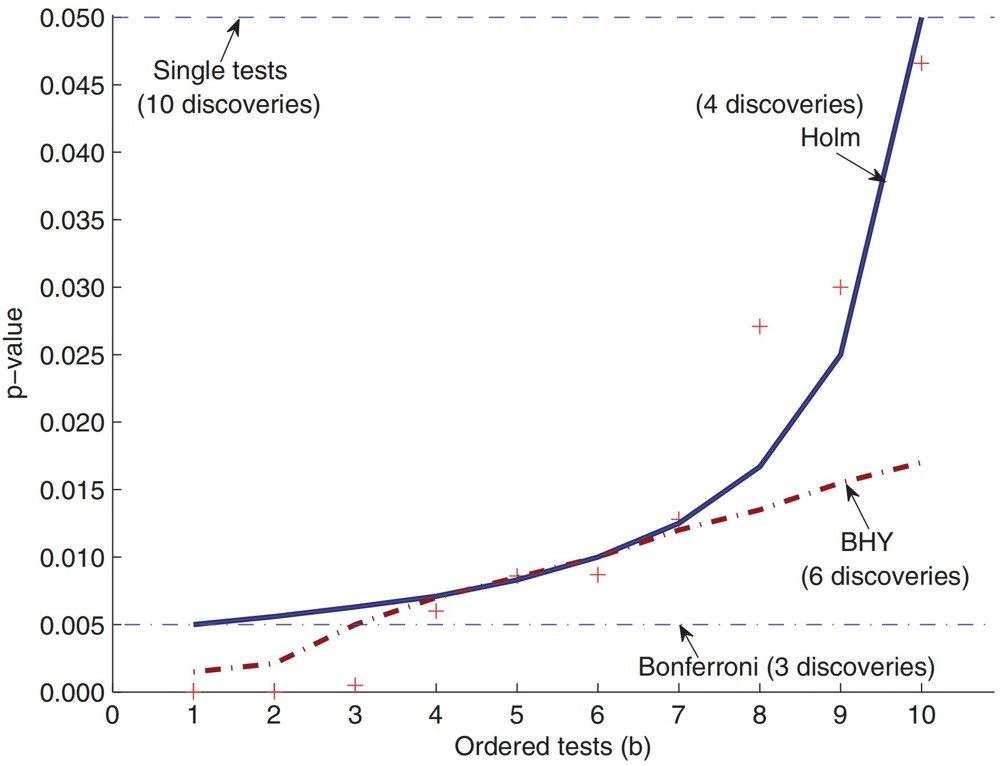
\includegraphics[width=0.85 \linewidth]
    	{pic/Multiple_test_thresholds.jpg}
%    \caption{}
  	\end{center}
	\end{figure}
\end{frame}
\begin{frame}{Adjusted t-statistics, 1965–2032}
	\begin{figure}[htpb]
  		\begin{center}
    	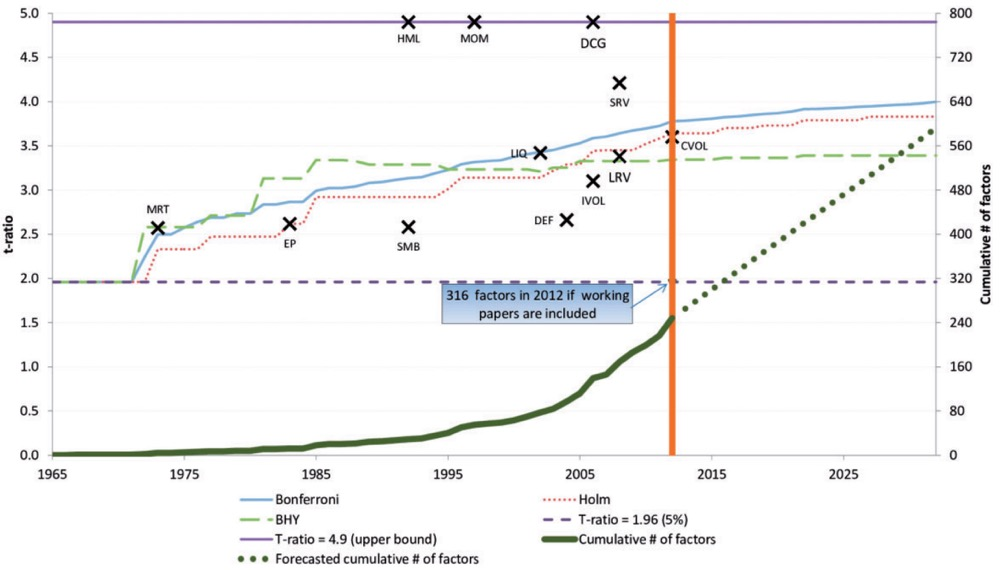
\includegraphics[width=1.05 \linewidth]
    	{pic/Adjusted-t-statistics.jpg}
	  	\end{center}
	\end{figure}
\end{frame}
\begin{frame}{An important Philosophical Issue and Conclusion}
	Why should we have a higher threshold for today’s data mining than for data mining in the 1980s?
	\begin{enumerate}
		\item The rate of \alert{discovering} a true factor has decreased.
		\item There is a limited amount of \alert{data} (CRSP database).
		\item The \alert{cost} of data mining has dramatically decreased.
	\end{enumerate}
	\\\ \\
	Many of the factors discovered in the field of finance are likely false discoveries: of the 296 published significant factors, 158 would be considered false discoveries under Bonferonni, 142 under Holm, 132 under BHY (1\%), and 80 under BHY (5\%)
\end{frame}

\section{Why Most Claimed Statistical Findings Are True}
\begin{frame}{``easy bound" on $\mathrm{FDR}_{|t|>2}$}
%	When someone discovered that coins are more likely to land heads (i.e. the coin toss is not fair), then we have
	$$
	\begin{aligned} 
		\mathrm{FDR}_{|t|>2} 
		& \approx \underbrace{\operatorname{Pr}\left(F_{i}\mid |t_{i}|>2\right)}_{\text{the predictor is false when}\ t>2}
		 = \frac{
		{
		\operatorname{Pr}\left(\left|t_{i}\right|>2 \mid F_{i}\right)}
		}
		{
		\operatorname{Pr}\left(\left|t_{i}\right|>2\right)
		} 
		\operatorname{Pr}\left(F_{i}\right) 
		\\ \ \\
		& \leq 
		\frac{
		\underbrace{\operatorname{Pr}\left(\left|t_{i}\right|>2 \mid F_{i}\right)}_{t>2 \ \text{when the predictor is false}}
		}{\operatorname{Pr}\left(\left|t_{i}\right|>2\right)}  
		 \approx \frac{5 \%}
		{\operatorname{Pr}\left(\left|t_{i}\right|>2\right)}
	\end{aligned}
	$$
	\begin{itemize}
		\item One might estimate $\operatorname{Pr}\left(\left|t_{i}\right|>2\right)$ by just counting the share of $|t_i|>2$.
		\item Since publication bias, $\operatorname{Pr}\left(\left|t_{i}\right|>2\right)$ may be overstated.
		\item This problem can be addressed by considering \alert{worst-case scenarios}.
	\end{itemize}
\end{frame}

\begin{frame}{Bounding the FDR using Data-Mining as a Worst-Case}
	\begin{figure}[htpb]
  		\begin{center}
    	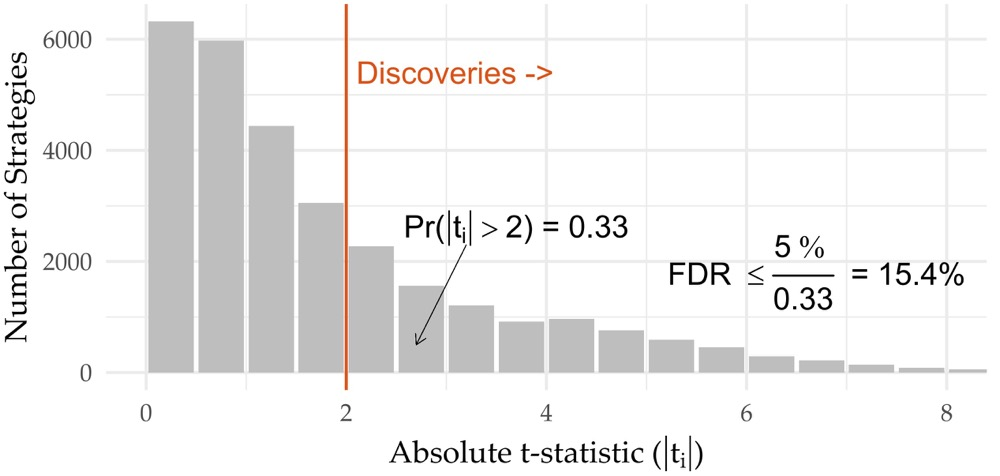
\includegraphics[width=0.9 \linewidth]
    	{pic/Data-Mining.jpg}
  		\end{center}
	\end{figure}
	\begin{center}
		Thus, at least 84.6\% of published predictors are true.
	\end{center}
\end{frame}

\begin{frame}{Bounding the FDR with Conservative Extrapolation}
	\begin{figure}[htpb]
  		\begin{center}
    	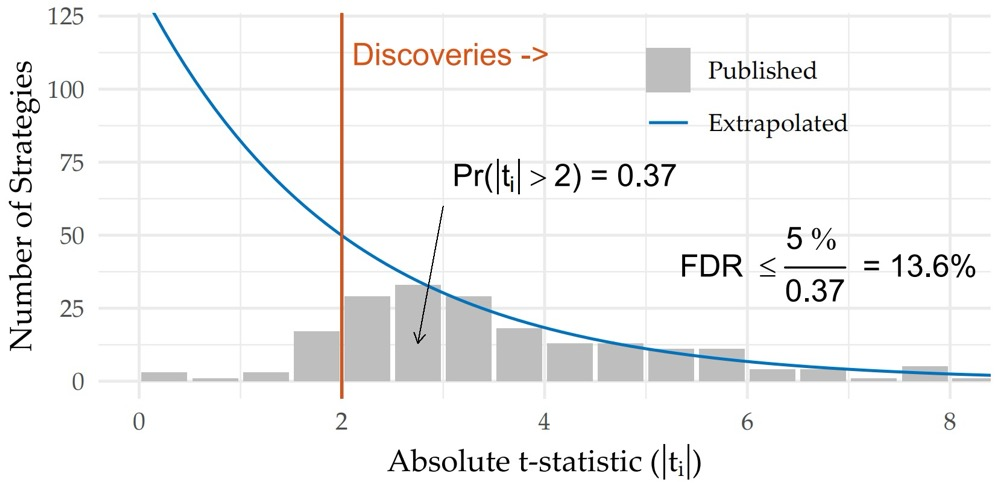
\includegraphics[width=0.9 \linewidth]
    	{pic/Conservative_Extrapolation.jpg}
  		\end{center}
	\end{figure}
	$$
	\mathrm{FDR}_{|t|>2} \leq \frac{5 \%}{\exp \left[-2 / \mathbb{E}\left(\left|t_{i}\right|\right)\right]}=\frac{5\%}{0.37}=13.6 \% \
	(\text{exponential CDF})
	$$
	\\
	$$
	\mathbb{E}\left(\left|t_{i}\right|\right)=\mathbb{E}\left(\left|t_{i}\right|\mid| t_{i}|>2\right)-2 \quad
	(\text{Due to the memoryless property})
	$$
\end{frame}

\begin{frame}{Two Interpretations of ``False Factor"}
\begin{multicols}{2}
	\begin{figure}[htpb]
  		\begin{center}
    	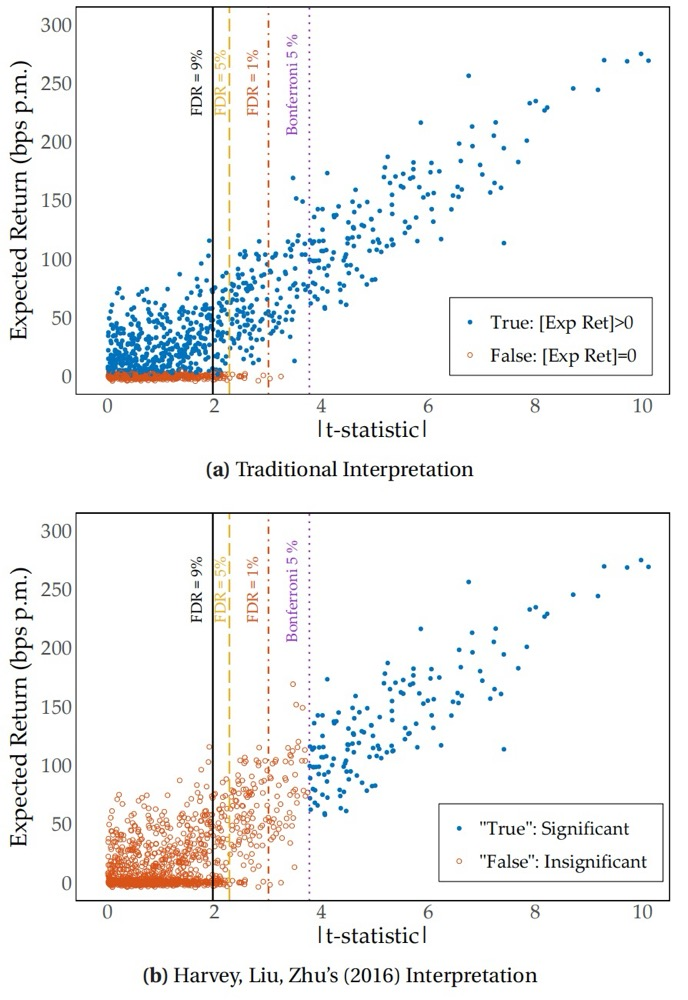
\includegraphics[width=0.88 \linewidth]
    	{pic/SMM.jpg}
  		\end{center}
	\end{figure}
	\begin{itemize}
		\item HLZ’s estimates imply $\mathrm{FDR}_{|t|>2} \approx 9 \%$
		\item why do they (HLZ) argue that ``most ... are more likely false?"
		\item ``false factor" vs ``insignificant factor"  (158/296=53\%)
		\item ``most" vs ``many" (80/296=27\%)
		\item ``null" vs ``insignificant"
	\end{itemize}
\end{multicols}
\end{frame}
%%%%%%%%%%%%%%%%%%%%%%%%%%
\begin{frame}{From ``Factor War" to ``Test War"}
	\begin{itemize}
		\item Lo and MacKinlay (1990): Data snooping can cause problems in testing asset pricing models.
		\item Sullivan et al. (1999): How to correct the impact of data snooping bias
		\item Harvey et al. (2016): After excluding the impact of multiple hypothesis testing, ``the vast majority" fail to achieve significant excess returns.
		\item Linnainmaa and Roberts (2018): Constructe new out-of-sample data to test.
		\item Chordia et al. (2020): Creative use of simulation methods to infer how statistical characteristics of study-based factor sets can eliminate the effects of multiple hypothesis testing。
	\end{itemize}
\end{frame}
% End
\begin{frame}[allowframebreaks]%{End}
	\begin{center}
		\Huge\textbf{\textit{\texttt{Thanks!}}}
	\end{center}
\end{frame}

% Reference
%\appendix
%\begin{frame}{Reference}
%	\addtocounter{framenumber}{-1}
%	\printbibliography % [heading=bibintoc, title=Reference]
%\end{frame}

%%%%%%%%%%%%%%%%%%%%%%%%%%

% Snippets
%\begin{frame}[noframenumbering, plain]{Snippets}
%	\begin{multicols}{2}
%		\begin{enumerate}
%			\item \cite[Page10]{barro1990}
%			\item parencite \\ \parencite{Greiner2008}
%			\item footcite \footcite{green2020}
%			\item \cite{Greiner2008}
%		\end{enumerate}
%		\begin{itemize}
%			\item \[V = \frac{4}{3}\pi r^3\]
%			\item $ V = \frac{4}{3}\pi r^3 $
%		\end{itemize}
%	\end{multicols}	
%	\begin{equation}
%		\label{eq1}
%		V = \frac{4}{3}\pi r^3
%	\end{equation}
%	\center 
%	As Equation(\ref{eq1}) shows, $\cdots$, this \emph{equation} is \alert{important}.
%\end{frame}
%
%
%
%\begin{frame}[noframenumbering, plain]{Snippets}
%	\begin{columns}
%		\column{0.5\textwidth}
%			\begin{block}{Remark}
%				Sample text
%			\end{block}
%			\begin{alertblock}{Important theorem}
%				Sample text in red box
%			\end{alertblock}
%			\begin{examples}
%				Sample text in green box. 
%			\end{examples}
%		\column{0.5\textwidth}
%			\begin{table}
%			    \centering
%			    \caption{table1}
%			    \vspace{-0.5cm}
%			    \setlength{\tabcolsep}{5mm}
%				    {
%				    \begin{tabular}{lcc}
%				    \hline
%			        123 & 123 & ad f \\ \hline
%			        \textcolor{deepred}{123} & w & ad f \\ 
%			        \textcolor{sufered}{123} & \alert{ad} f & ad s f \\ \hline
%				    \end{tabular}
%				    }
%			    \label{fig1}
%			\end{table}
%	\end{columns}
%\end{frame}
%\backupend
%%%%%%%%%%%%%%%%%%%%%%%%%%
\end{CJK*}
\end{document}
